\documentclass[12pt,a4paper]{extreport}
\usepackage[utf8]{inputenc}
\usepackage[french]{babel}
\usepackage[T1]{fontenc}
\usepackage{amsmath}
\usepackage{amsfonts}
\usepackage{amssymb}
\usepackage{graphicx}
\author{Sébastien Hervieu}
\title{ Inverse Problems: Tomography Project}
\renewcommand{\thesection}{\alph{section}}
\begin{document}
\maketitle
\section{Question 1}
\paragraph*{}
The algorithm for generating the $G$ matrix for a $Nx \times Ny$ model, using the requested ray geometry, is implemented in a Matlab function called $computeG(Nx,Ny)$, which is in the $computeG.m$ file.

\paragraph*{}
The algorithm includes two main parts:
\begin{itemize}
\item The first part handles the generation of the horizontal and vertical rays;
\item The second part handles the generation of the diagonal rays.
\end{itemize}

\paragraph*{}
The implementation of the first part (lines 10 to 26) is very straightforward.

\paragraph*{}
The second part is much more complex and requires an adequate analysis of the relations of the rays between each other. We notice that for each direction of diagonal rays there is a relation between one ray and the next one.

\paragraph*{}
For example, for the rays going diagonaly up from the left, the first ray only goes through the first cell of the first row of the model. Then the second ray, goes through the first cell of the second row, and then to the second cell of the first row, and so one.

\paragraph*{}
We use these relations to implement an algorithm based on shifting and stacking lines (such as in lines 36 to 54).

\paragraph*{}
We then handle the case of $Nx \neq Ny$ in two different ways:
\begin{itemize}
\item for the up diagonals, we check if the current ray start line number is higher or not than $Ny$ (line 37), in which case we just insert a blank line to the top and remove the bottom line from the previous ray (lines 42 and 45);
\item for the down diagonals, we check if the current ray start column number is higher or not than $Nx - Ny +1$ (line 60), in which case we add a blank line to the top and remove the bottom line from the previous lines (lines 66 to 70).
\end{itemize} 

\paragraph*{}
When the ray model matrix is complete (size $Nx \times Ny$), we then transform this matrix to row vector and add it to the bottom of the $G$ matrix (for example lines 48 to 62).

\section{Question 2}
Using 7 x 7 the spike model, by running the provided $Q2ComputeWithSpike.m$ script, we generate the $G$ matrix $d$.

We then reconstruct the model based on various noise level on the data and we get the following results:
\begin{figure}[h]
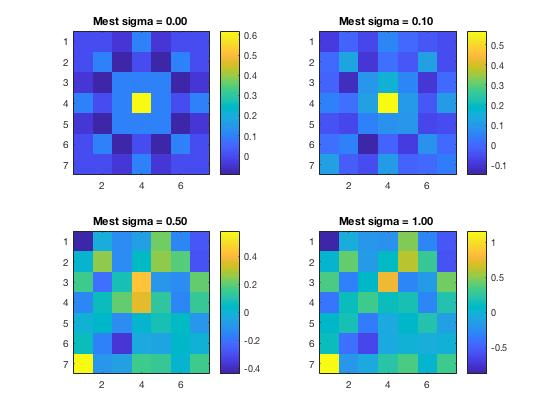
\includegraphics[width=15cm]{Q2Image.jpg} 
\caption{Result with Spike Model $Nx=Ny=7$}
\end{figure}

\paragraph*{}
We notice that the spike in the center is very well reconstructed in the case without noise, but that there is a kind of "spread" of the spike in the remainder of the model.

\paragraph*{}
As the noise increases, the model reconstruction is degraded, up to the point it is not recognisable at $\sigma = 1$.

\section{Question 3}
We reproduce the previous experiment with  $Nx = Ny = 11, 15$ and $21$, by running the scripts $Q3ComputeWithSpike11.m$, $Q3ComputeWithSpike15.m$ and $Q3ComputeWithSpike21.m$ respectively.

\paragraph*{}
We get the following results, first for $Nx=Ny=11$

\begin{figure}[h]
\includegraphics[width=15cm]{Q3Spike11.jpg} 
\caption{Result with Spike Model $Nx=Ny=11$}
\end{figure}
\newpage
then for $Nx=Ny=15$,

\begin{figure}[h]
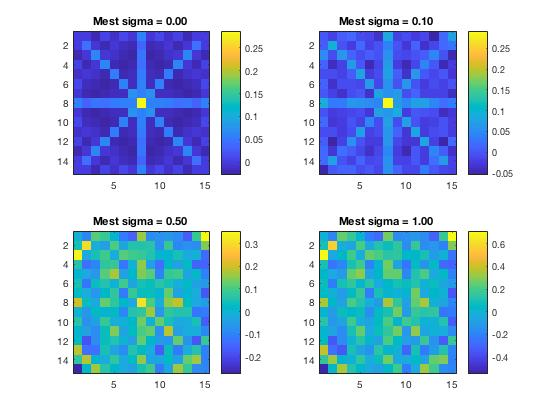
\includegraphics[width=15cm]{Q3Spike15.jpg} 
\caption{Result with Spike Model $Nx=Ny=15$}
\end{figure}

\newpage
and finally for $Nx=Ny=21$
 
\begin{figure}[h]
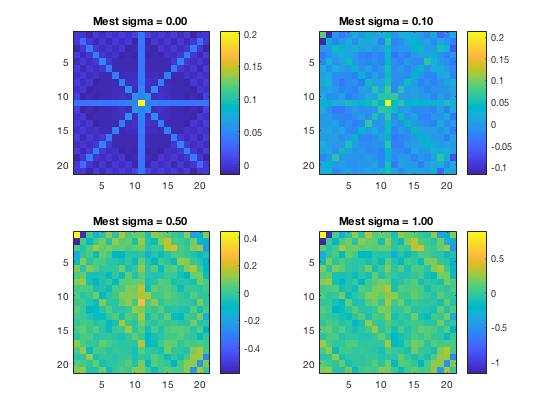
\includegraphics[width=15cm]{Q3Spike21.jpg} 
\caption{Result with Spike Model $Nx=Ny=21$}
\end{figure}

We see that as the size of the model increases, it becomes more and more sensitive to the noise, as the relative noise level become higher as there is more data for bigger model, and the spike signal gets drowned in the resulting noise.

\newpage

\section{Question 4}

We choose to use 2 different graphic files to test with a more complex model. 
The first one is a simple 15x15 black and white "Invader" sprite:
\begin{figure}[h]
\begin{center}

\includegraphics[width=8cm]{../invader15x15.png} 
\end{center}
\caption{Invader model $Nx=Ny=15$}
\end{figure}

\newpage

The second model is handmade "Mario" model, with 5 different levels of grey:
\begin{figure}[!h]
\begin{center}

\includegraphics[width=8cm]{../mario16x16.png} 
\end{center}
\caption{Mario model $Nx=Ny=16$}
\end{figure}

The requested computation is performed on the "Invader" model by executing the $Q4ComputeWithInvader.m$ scripts.
\newpage
The results for the Invader model are shown below.

\begin{figure}[h]
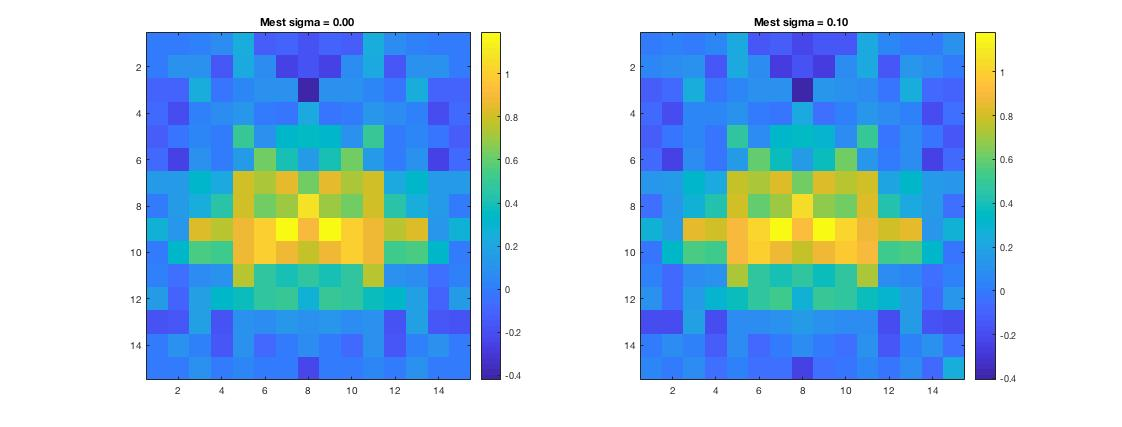
\includegraphics[width=15cm]{InvaderResult.jpg} 
\caption{Result with Invader Model $Nx=Ny=15$}
\end{figure}

We can see from that the model reconstruction works quite well, as the shape of the invader is recognisable at both $\sigma$. However the small border details are attenuated when compared to the original model.

\newpage
The computations for the Mario model are performed by running the $Q4ComputeWithMario.m$ script from matlab.

The results for the Mario are shown below:
\begin{figure}[h]
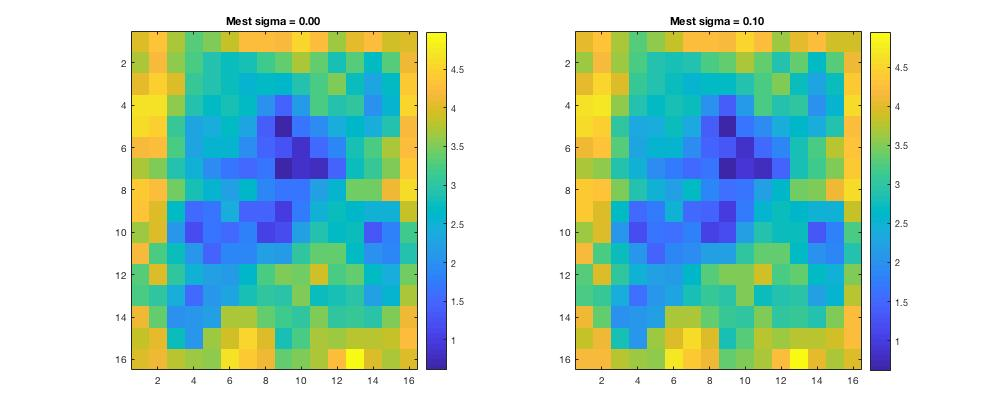
\includegraphics[width=15cm]{MarioResults.jpg} 
\caption{Result with Mario Model $Nx=Ny=16$}
\end{figure}

Once again the global shape of the original model is recognizable but the details are mostly blurred in the background.
\newpage
\section{Question 5}
In order to build the increased resolution, we use a small custom function that takes in the model in the original resolution and outputs the  higher resolution model ($tripleBitmap.m$).

\paragraph*{}
To perform the computation for the Invader model in higher resolution, we use the $Q5ComputeWithInvader_x3.m$ script.
The results are shown below:

\begin{figure}[h]
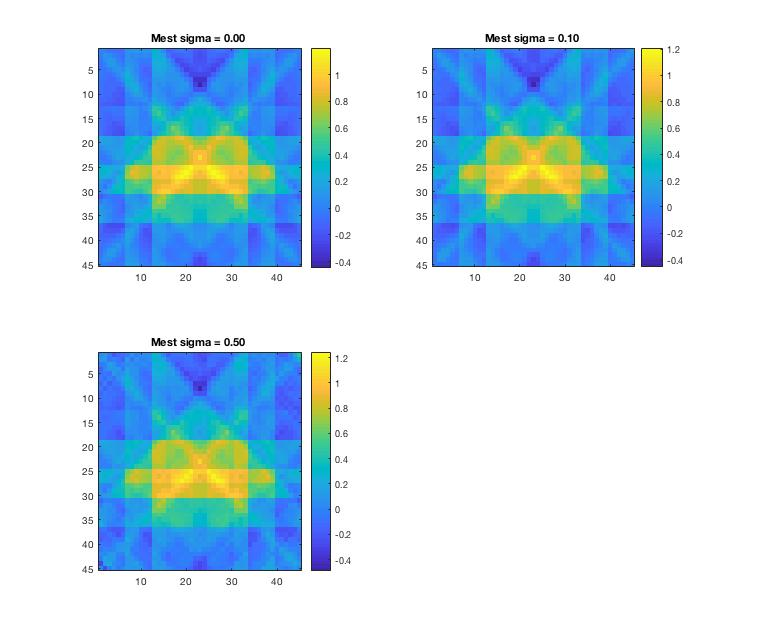
\includegraphics[width=15cm]{InvaderResults3x.jpg} 
\caption{Result with Invader Model with 3 times more resolution$Nx=Ny=45$}
\end{figure}

We can see that the model is reconstructed in sligthly more details inside the model, the image is more contrasted, especially inside the body of the mode, the holes representing rhe "eyes" are especially visible. However details such as the "arms" are not all reconstructed.

\paragraph*{}
The computation for the Mario model in higher resolution is performed by launching the $Q5ComputeWithMario_x3.m$ script.
\
The results are displayed below:

\begin{figure}[h]
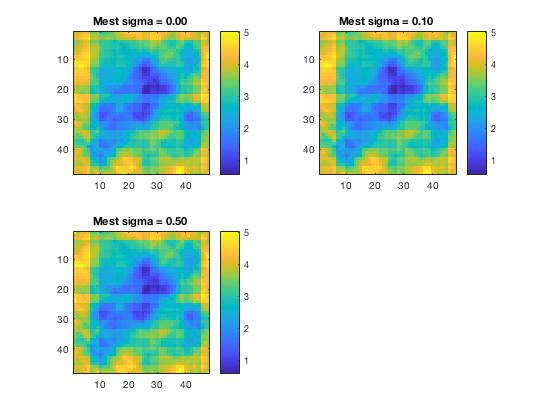
\includegraphics[width=15cm]{MarioResults3x.jpg} 
\caption{Result with Mario Model with 3 times the original resolution.$Nx=Ny=48$}
\end{figure}
Once again, holes inside the model well detected, but the precise shape is mostly lost.

\newpage
\section{Question 6} 
In order to generate a G matrix from a rectangular model, one need to call the generateG function with matrix M as input.

\paragraph*{}
To generate data from a G matrix, use the generateDataFromModel() function, which takes in the data G matrix of the model.

\paragraph{}
To reconstruct a model from a data vector, use the computeModelFromData() function, which takes in the d data vector and the G matrix and return a reconstructed model in the form of a vector.

\paragraph{}
Then pass the model vector to the rebuildModel() function, to restitute the geometry of the model ($Nx$ and $Ny$ need to be known).

\end{document}